\documentclass[11pt, a4paper, twocolumn]{article}


% --- Paquetes de Idioma y Codificación ---
\usepackage[utf8]{inputenc}
\usepackage[spanish, es-nodecimaldot]{babel} % Configurado para español
\usepackage[T1]{fontenc}

% --- Tipografía y Estética ---
\usepackage{mathpazo} % Fuente Palatino, elegante y legible
\usepackage{microtype} % Mejora el espaciado entre letras y palabras

% --- Geometría de Página ---
\usepackage[margin=2.5cm, top=3.8cm, headheight=65pt, headsep=0.8cm]{geometry}
\columnsep 0.6cm % Espacio entre columnas

% --- Matemáticas Avanzadas ---
\usepackage{amsmath, amsfonts, amssymb, amsthm}
\usepackage{mathtools}

% --- Gráficos y Tablas ---
\usepackage{graphicx}% Para incluir imágenes
\usepackage{booktabs} % Para tablas con estilo profesional (sin líneas verticales)
\usepackage{caption}
\usepackage{float} % Permite el uso del modificador [H] para fijar la posición de las tablas
\captionsetup{labelfont=bf, font=small} % Captions en negrita y pequeñas

% --- Hipervínculos y Referencias ---
\usepackage[colorlinks=true, allcolors=blue]{hyperref}
\usepackage[capitalize]{cleveref} % Referencias inteligentes (ej: Fig. 1)
\usepackage{csquotes} % Soluciona el warning de babel/polyglossia
\usepackage{biblatex}
\addbibresource{difraccion.bib}

% --- Título y Autores ---
\title{\textbf{\Large Difracción: Estudio Experimental y Espectroscópico}}
\author{
    \textbf{Truchado Iniesta, Eduardo}, \textbf{Sanz Rubio, Juan} \\
    \small Grado de Física, UCLM. \texttt{juan.sanz1@alu.uclm.es} \\
    \small Grado de Física, UCLM. \texttt{eduardo.truchado@alu.uclm.es}
}
\date{\small 2 Marzo 2026}


\usepackage{fancyhdr}
%\usepackage{graphicx}

% --- Configuración del Encabezado ---
\pagestyle{fancy}
\fancyhf{} % Limpia encabezado y pie de página
\renewcommand{\headrulewidth}{0.4pt} % Línea horizontal bajo el encabezado

% Imagen a la IZQUIERDA
\fancyhead[L]{
\includegraphics[height=2cm]{logoFCTo.png}}

\fancyfoot[C]{\thepage}


\fancypagestyle{plain}{
    \fancyhf{} % Limpia el estilo plain por defecto
    \fancyhead[L]{
\includegraphics[height=2cm]{logoFCTo.png}} % Mantiene tu logo
    \fancyfoot[C]{\thepage} % Fuerza el número de página
    \renewcommand{\headrulewidth}{0.4pt} % Mantiene la línea
}

% --- Inicio del Documento ---

\begin{document}
\sloppy

\maketitle
\thispagestyle{fancy}

%Resumen

\begin{abstract}
En esta práctica, se realizan 3 partes. La primera de ellas se trata de usando la medición de los máximos y mínimos del patrón 
de difracción generado, se mida la anchura de una rendija que genera el patrón, en este primer caso se utiliza una rendija simple. 
Después en la segunda parte se realiza el mismo cálculo pero para una red de difracción así pudiendo obtener su parámetro de red. 

\vspace{0.2cm}

A parte se ha realizado una parte opcional donde se consigue un patrón de difracción circular a través de un filtro con aberturas circulares. Y por último se analizan las 
longitudes de onda espectroscópicas del helio a través de la red de difracción analizada previamente. 
\end{abstract}



\section{Introducción}
La difracción es un efecto físico propio de las ondas que ocurre cuando estas chocan contra un obstáculo cuya anchura
es similar a la $\lambda$ de la misma. En este caso el obstáculo se vuelve un nuevo foco de ondas secundario que en el 
caso de existir varios de estos, como en el estudio aquí realizado, generaran patrones de interferencia. 

\vspace{0.2cm}

En nuestro caso nos es de interés el patrón de difracción de \textit{Franhoufer}, es decir a una distancia considerable de la 
fuente principal. Así, la intensidad de la luz viene dada por la siguiente relación: 

\begin{equation}
    I \sim \frac{sin(\beta^{2})}{\beta^{2}}
\end{equation}
Donde $\beta = k a sin(\theta)$. 

\vspace{0.2cm}

Por otro lado en este estudio también se realizará un tratamiento espectroscópico a un elemento químico. Cada uno de estos 
emite un espectro de longitudes de onda característico que nos permite identificarlo bajo una emisión de luz y usando una red 
de difracción como filtro.


\section{Objetivos}
El objetivo principal de esta práctica es el estudio de la difracción para diferntes tipos de obstáculos y como esta difracción puede
 ayudarnos a analizar la composición de elementos químicos al actuar como un filtro de luz que deja pasar solo las longitudes de onda que deseamos.
\section{Metodología}
 
Para el estudio aquí presentado se han realizado mediciones del patrón de difracción tras colocar el láser con $\lambda = 630-650 nm$ frente a la red de
difraccición. Esta a su vez se ha colocado a una distancia variable de entre 0.3 a 1 metro de respecto a la pantalla donde se han tomado las medidas, en este caso una caja de cartón.
Estas medidas se han tomado con un calibre milimetrado. Con estos datos usaremos la relación de intensidad mostrada antes para llegar a la relación: 

\begin{equation}
    2 a sin(\theta) = m \lambda
\end{equation}

Donde si aproximamos $sin(\theta) \approx \theta = \frac{D}{L}$:

\begin{equation}
    X_{min} = \frac{\lambda D}{2 a}
\end{equation}

Y donde $2a$ es la anchura de la rendija, $D$ es la distancia entre los mínimos y $L$ es la distancia entre la rendija y la pantalla. Para una red de difracción es casi igual cambiando la distancia 
$2a$ por el parámetro de red $\frac{1}{2d}$ (en líneas/mm).

\begin{figure}[h]
    \centering
    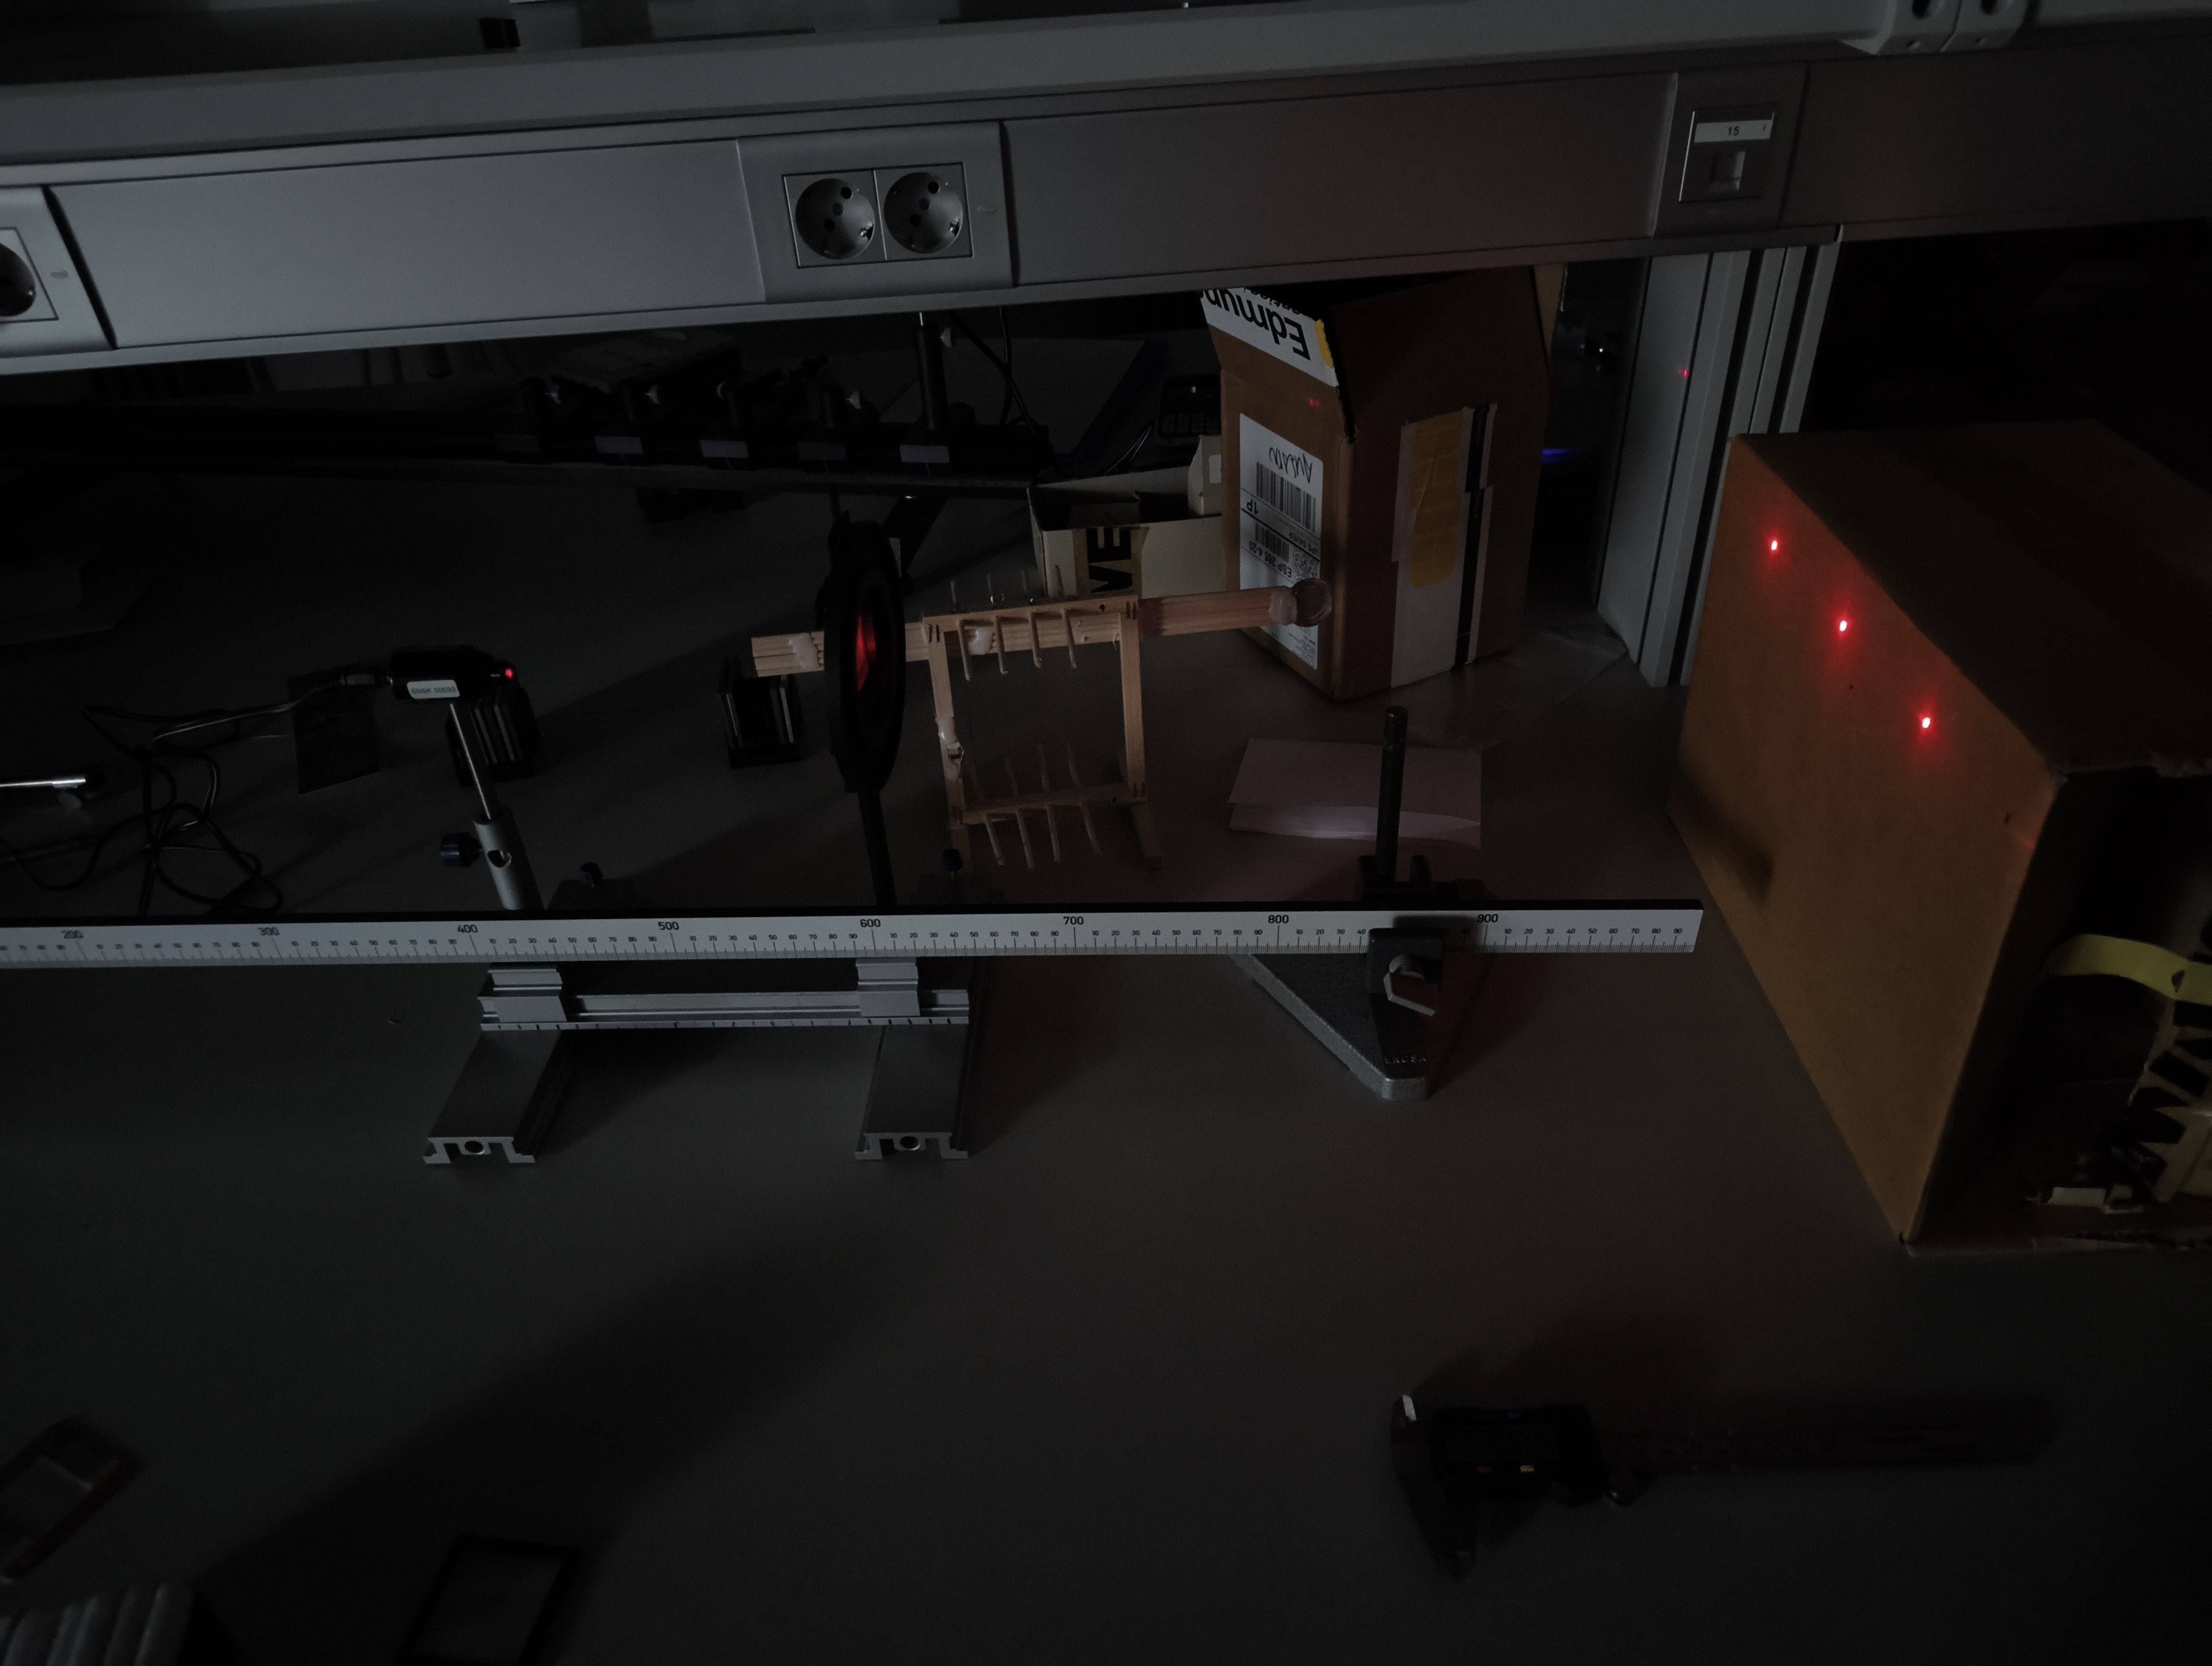
\includegraphics[width=0.4\textwidth]{fotos_practica/montaje_rendija.jpg}
    \caption{Montaje para el estudio de la difracción}
\end{figure}

Posterioremnte para el estudio espectroscópico se ha colocado la red en un goniómetro apuntando en la dirección de la emisión de luz de la lámpara del helio. Con el goniómetro se han calculado 
los ángulos respecto a un ángulo incial de referencia y con estos datos se han realizado los cálculos usando la siguiente relación: 

\begin{equation}
    \theta_{i} = arcsin\left(\frac{\lambda_{i}}{2d}\right) \approx \frac{\lambda_{i}}{2d}
\end{equation}


\begin{figure}[h]
    \centering
    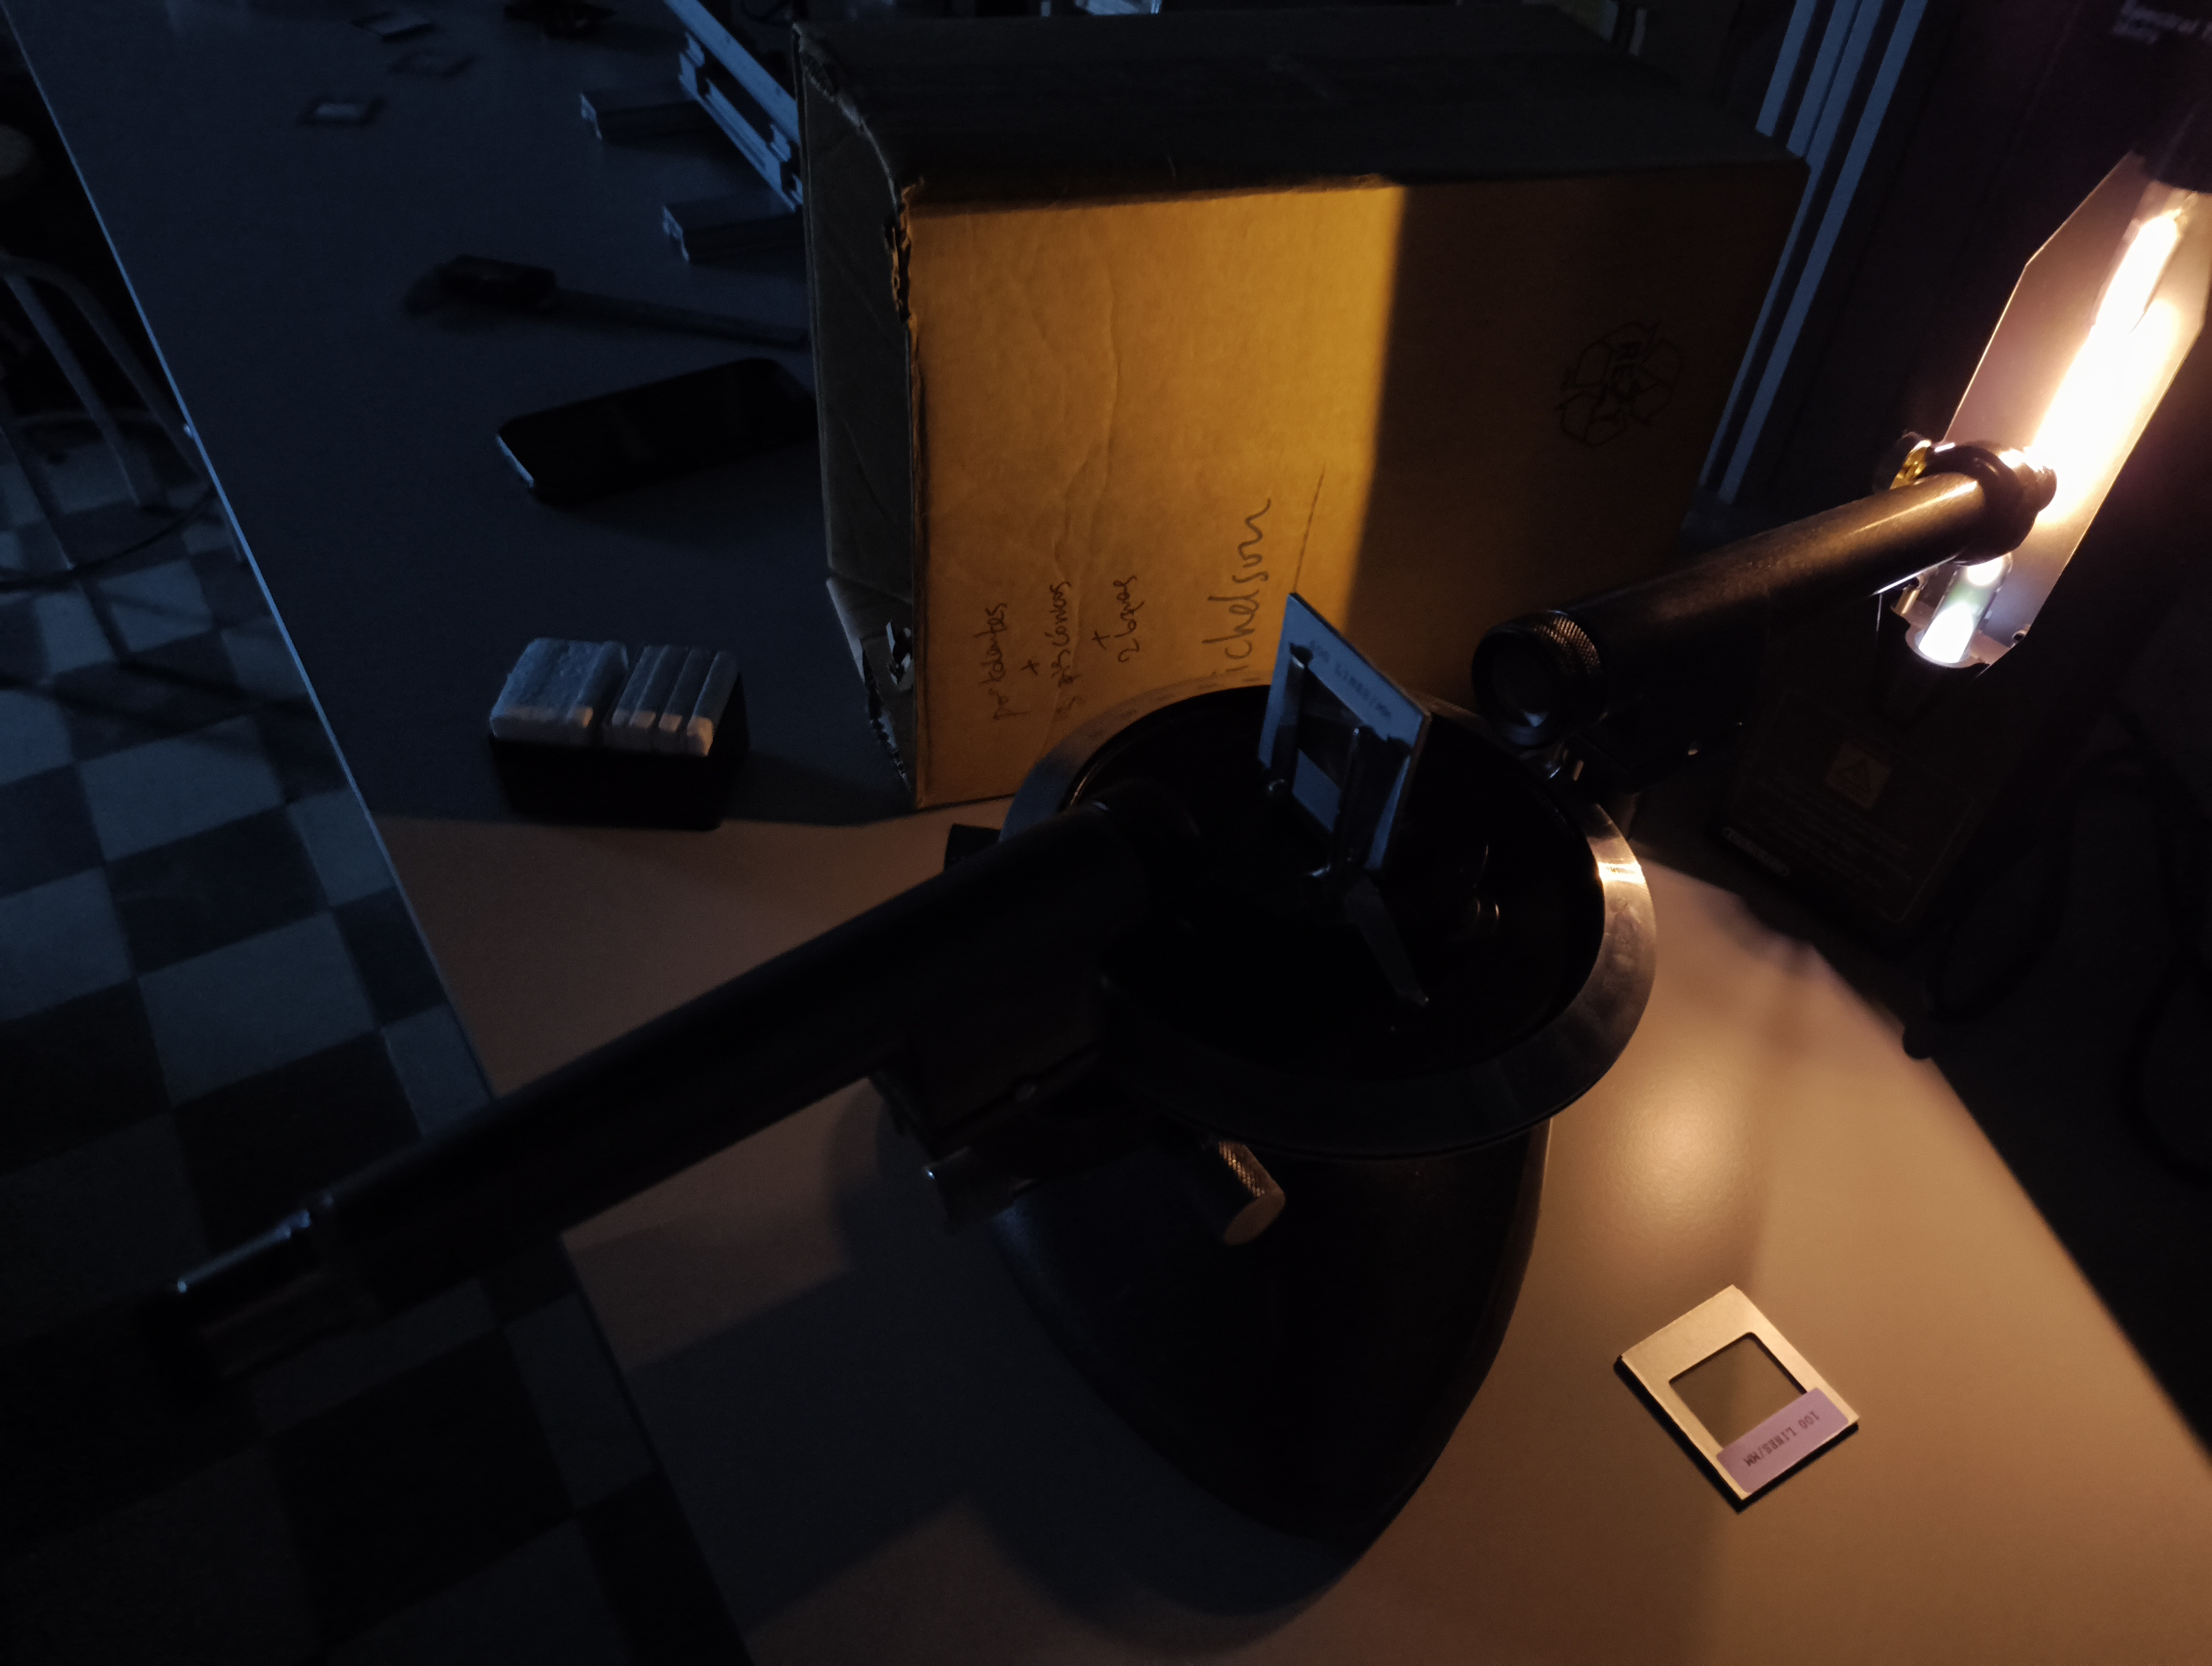
\includegraphics[width=0.4\textwidth]{fotos_practica/montaje_espectroscopio.jpg}
    \caption{Montaje para el estudio espectroscópico}
\end{figure}

\section{Tratamiento de datos}
\subsection{Rendija simple}
Tomamos las medidas de la anchura del patrón de difracción 5 veces para cada caso. La distancia mostrada es la medida entre los dos primeros mínimos, $m = -1$ y $m=1$ dividida entre 2 para reducir errores.

\begin{table}[H]
    \caption{Tabla para la toma 1 }
    \centering
    \small
    \setlength{\tabcolsep}{4pt}
    \begin{tabular}{cccc}
        \hline
        $D$ (mm) &   $X_{min}$ (mm) & $\Delta D$ (mm) & $\Delta X_{min}$ (mm)  \\
        \hline
            1000 &       4.5   & $\pm 0.02$   & $\pm 0.01$    \\
            900 &       4.06  & $\pm 0.02$    & $\pm 0.01$    \\
            800 &       3.43  & $\pm 0.02$    & $\pm 0.01$   \\
            700 &       3.18 & $\pm 0.02$    & $\pm 0.01$   \\
            600 &       2.53 & $\pm 0.02$    & $\pm 0.01$   \\
        \hline
    \end{tabular}
\end{table}

\vspace{0.5cm}

\begin{table}[H]
    \caption{Tabla para la toma 2 }
    \centering
    \small
    \setlength{\tabcolsep}{4pt}
    \begin{tabular}{cccc}
        \hline
        $D$ (mm) &   $X_{min}$ (mm) & $\Delta D$ (mm)  & $\Delta X_{min}$ (mm)  \\
        \hline
            1000 &       5.33  & $\pm 0.02$    & $\pm 0.01$    \\
            900 &       4.79 & $\pm 0.02$    & $\pm 0.01$    \\
            800 &       4.06  & $\pm 0.02$    & $\pm 0.01$   \\
            700 &       3.89  & $\pm 0.02$    & $\pm 0.01$   \\
            600 &       2.94 & $\pm 0.02$    & $\pm 0.01$   \\
        \hline
    \end{tabular}
\end{table}


\vspace{0.5cm}

\begin{table}[H]
    \caption{Tabla para la toma 3 }
    \centering
    \small
    \setlength{\tabcolsep}{4pt}
    \begin{tabular}{cccc}
        \hline        
        $D$ (mm) &   $X_{min}$ (mm) & $\Delta D$ (mm)   & $\Delta X_{min}$ (mm)  \\
        \hline
            1000 &       6.74  & $\pm 0.02$        & $\pm 0.01$\\
            900 &       6.11 & $\pm 0.02$        & $\pm 0.01$\\
            800 &       5.42 & $\pm 0.02$        & $\pm 0.01$\\
            700 &       4.82 & $\pm 0.02$        & $\pm 0.01$\\
            600 &       3.95 & $\pm 0.02$        & $\pm 0.01$\\
        \hline
    \end{tabular}

\end{table}

\vspace{0.5cm}

\begin{table}[H]
    \caption{Tabla para la toma 4 }
    \centering
    \small
    \setlength{\tabcolsep}{4pt}
    \begin{tabular}{cccc}
        \hline
        $D$ (mm) &   $X_{min}$ (mm) & $\Delta D$ (mm)   & $\Delta X_{min}$ (mm)  \\
        \hline
            1000 &       8.9   & $\pm 0.02$   & $\pm 0.01$ \\
            900 &       7.68  & $\pm 0.02$    & $\pm 0.01$ \\
            800 &       7.14  & $\pm 0.02$    & $\pm 0.01$ \\
            700 &       6.06  & $\pm 0.02$    & $\pm 0.01$ \\
            600 &       5.47 & $\pm 0.02$    & $\pm 0.01$ \\
        \hline
    \end{tabular}
\end{table}

\vspace{0.5cm}

\begin{table}[H]
    \caption{Tabla para la toma 5 }
    \centering
    \small
    \setlength{\tabcolsep}{4pt}
    \begin{tabular}{cccc}
        \hline
        $D$ (mm) &   $X_{min}$ (mm) & $\Delta D$ (mm)  & $\Delta X_{min}$ (mm) \\
        \hline
            1000 &      12.15 & $\pm 0.02$   & $\pm 0.01$    \\
            900 &      10.66  & $\pm 0.02$    & $\pm 0.01$   \\
            800 &       9.91  & $\pm 0.02$    & $\pm 0.01$   \\
            700 &       8.89  & $\pm 0.02$    & $\pm 0.01$   \\
            600 &       6.92 & $\pm 0.02$    & $\pm 0.01$   \\
        \hline
    \end{tabular}

\end{table}

\vspace{0.5cm}

\begin{table}[H]
    \caption{Tabla para la toma 6 }
    \centering
    \small
    \setlength{\tabcolsep}{4pt}
    \begin{tabular}{cccc}
        \hline
        $D$ (mm) &   $X_{min}$ (mm) & $\Delta D$ (mm)  & $\Delta X_{min}$ (mm)\\
        \hline
            1000 &      31.3   & $\pm 0.02$   & $\pm 0.01$    \\
            900 &      28.13 & $\pm 0.02$   & $\pm 0.01$    \\
            800 &      25.17  & $\pm 0.02$   & $\pm 0.01$    \\
            700 &      22.09 & $\pm 0.02$   & $\pm 0.01$    \\
            600 &      18.79 & $\pm 0.02$   & $\pm 0.01$    \\
        \hline
    \end{tabular}
\end{table}

\subsection{Red de difracción}
Para el caso de una red de difracción, se han examinado 3 redes distintas para buscar sus parámetros de red y obtener el número de líneas por milímetro:

\begin{table}[H]
    \caption{Tabla para la red de 600 líneas/mm }
    \centering
    \small
    \setlength{\tabcolsep}{4pt}
    \begin{tabular}{cccc}
        \hline
        $D$ (mm) &   $X_{max}$ (mm) & $\Delta D$ (mm)   & $\Delta X_{max}$ (mm)   \\
        \hline
            350 &            140   & $\pm 0.5$         & $\pm 0.5$               \\
            300 &            126   & $\pm 0.5$         & $\pm 0.5$               \\
            250 &             98   & $\pm 0.5$         & $\pm 0.5$               \\
            200 &             79.5 & $\pm 0.5$         & $\pm 0.5$               \\
            150 &             60   & $\pm 0.5$         & $\pm 0.5$               \\
        \hline
    \end{tabular}

       
\end{table}

\vspace{0.5cm}

\begin{table}[H]
    \caption{Tabla para la red de 300 líneas/mm}
    \centering
    \small
    \setlength{\tabcolsep}{4pt}
    \begin{tabular}{cccc}
        \hline
        $D$ (mm) &   $X_{max}$ (mm) & $\Delta D$ (mm)   & $\Delta X_{max}$ (mm)   \\
        \hline
            700 &            142   & $\pm 0.5$         & $\pm 0.5$               \\
            600 &            119   & $\pm 0.5$         & $\pm 0.5$               \\
            500 &            101   & $\pm 0.5$         & $\pm 0.5$               \\
            400 &             75   & $\pm 0.5$         & $\pm 0.5$               \\
            300 &             59.5 & $\pm 0.5$         & $\pm 0.5$               \\
        \hline
    \end{tabular}
\end{table}

\vspace{0.5cm}

\begin{table}[H]
    \caption{Tabla para la red de 100 líneas/mm}
    \centering
    \small
    \setlength{\tabcolsep}{4pt}

    \begin{tabular}{cccc}
        \hline
        $D$ (mm) &   $X_{max}$ (mm) & $\Delta D$ (mm)   & $\Delta X_{max}$ (mm)   \\
        \hline
            700 &             45.5 & $\pm 0.5$         & $\pm 0.5$               \\
            600 &             42   & $\pm 0.5$         & $\pm 0.5$               \\
            500 &             30.5 & $\pm 0.5$         & $\pm 0.5$               \\
            400 &             25   & $\pm 0.5$         & $\pm 0.5$               \\
            300 &             19.5 & $\pm 0.5$         & $\pm 0.5$               \\
        \hline
    \end{tabular}

\end{table}

En este caso además, necesitamos calcular el error asociado a la medidada de $p = 1/2d$ a través de la relación $p = \frac{X_{max}}{D \cdot \lambda}$ que utilizaremos
más adelante en el estudio espectroscópico ya que uilizaremos los valores medios obtenidos de $p$ para el cálculo de las longitudes de onda del helio. Así, el error asociado a $p$ es el siguiente:

\begin{align}
    \Delta p &= \left|\frac{\partial p}{\partial X_{max}}\right|\Delta X_{max} + \left|\frac{\partial p}{\partial D}\right|\Delta D \\
    &= \frac{1}{D \cdot \lambda} \Delta X_{max} + \frac{X_{max}}{D^2 \cdot \lambda} \Delta D
\end{align}

\subsection{Parte opcional: Patrón de difracción circular}
En esta parte se ha realizado un estudio del patrón de difracción circular.

\subsection{Espectroscopía de un gas}

Tomamos las medidas de los ángulos de difracción con el goniómetro, en este caso contamos como ángulo de referecncia la marca de 324$^\circ$ en el goniómetro. 
Es importante hacer previamente el cálculo del error asociado a $\lambda$ a través de la relación $\lambda_{i} = \frac{\theta_{i}}{p}$ donde p es el parámetro de red caclulado previamente. 
Así el cálculo del error de $\lambda$ es el siguiente:

\begin{align}
    \Delta \lambda_{i} & = \left|\frac{\partial \lambda_{i}}{\partial \theta_{i}}\right|\Delta \theta_{i} + \left|\frac{\partial \lambda_{i}}{\partial p}\right|\Delta p \\
    & = \frac{1}{p} \Delta \theta_{i} + \frac{\theta_{i}}{p^2} \Delta p
\end{align}

Y los resultados obtenidos para cada red serán los siguientes:

\begin{table}[H]
    \caption{Tabla espectroscópica para la red de 100 líneas/mm}
    \centering
    \small
    \setlength{\tabcolsep}{4pt}
    \begin{tabular}{cccc}
        \hline
        $\theta_{i}$ (grados) &   $\lambda_{i}$ (nm) &   $\Delta \theta_{i}$ (grados) & $\Delta \lambda_{i}$ (nm)   \\
        \hline
                    0   &          0     &                     $\pm 0.01$ & $ \pm 0.0001$            \\
                    2.5 &        431.491 &                     $\pm 0.01$ & $ \pm 0.0001$            \\
                    3   &        517.716 &                     $\pm 0.01$ & $ \pm 0.0001$            \\
                    3.5 &        603.903 &                     $\pm 0.01$ & $ \pm 0.0001$            \\
                    4   &        690.043 &                     $\pm 0.01$ & $ \pm 0.0001$            \\
                    8   &       1376.72  &                     $\pm 0.01$ & $ \pm 0.0001$            \\
        \hline
    \end{tabular}
\end{table}

\vspace{0.5cm}
\begin{table}[H]
    \caption{Tabla espectroscópica para la red de 300 líneas/mm}
    \centering
    \small
    \setlength{\tabcolsep}{4pt}
    \begin{tabular}{cccc}
        \hline
        $\theta$ (grados) &   $\lambda$ (nm) & $\Delta \theta$ (grados)   & $\Delta \lambda$ (nm)   \\
        \hline
                        0   &            0     & $\pm$ 0.01                     & $\pm$ 3e-05                 \\
                        7.5 &          422.319 & $\pm$ 0.01                     & $\pm$ 3e-05                 \\
                        8   &          450.296 & $\pm$ 0.01                     & $\pm$ 3e-05                 \\
                        9   &          506.146 & $\pm$ 0.01                     & $\pm$ 3e-05                 \\
                        10   &          561.841 & $\pm$ 0.01                     & $\pm$ 3e-05                 \\
                        11.5 &          645.058 & $\pm$ 0.01                     & $\pm$ 3e-05                 \\
        \hline
    \end{tabular}
    
\end{table}

\vspace{0.5cm}

\begin{table}[H]
    \caption{Tabla espectroscópica para la red de 600 líneas/mm}
    \centering
    \small
    \setlength{\tabcolsep}{4pt}
    \begin{tabular}{cccc}
        \hline
        $\theta$ (grados) &   $\lambda$ (nm) & $\Delta \theta$ (grados)   & $\Delta \lambda$ (nm)   \\
        \hline
                        0   &            0     & $\pm$ 0.01                     & $\pm$ 2e-05                 \\
                        16   &          438.934 & $\pm$ 0.01                     & $\pm$ 2e-05                 \\
                        17   &          465.582 & $\pm$ 0.01                     & $\pm$ 2e-05                 \\
                        17.5 &          478.854 & $\pm$ 0.01                     & $\pm$ 2e-05                 \\
                        18   &          492.089 & $\pm$ 0.01                     & $\pm$ 2e-05                 \\
                        21   &          570.677 & $\pm$ 0.01                     & $\pm$ 2e-05                 \\
        \hline
    \end{tabular}
\end{table}

\section{Análisis de resultados}

Ahora procederemos a representar gráficamente los resultados ohbtenidos para en cada caso, obtener lo que se nos pide.

\subsection{Rendija simple}
En esta parte representaremos gráficamente la relación entre $X_{min}$ y $D$ para cada una de las 6 tomas realizadas. Además, se realizará un ajuste lineal a cada una de las gráficas para obtener el valor de $m$ 
y así poder obtener el valor de la anchura de la rendija. Para el cálculo, supondremos que el laser tiene una $\lambda = $

\begin{figure}[H]
    \centering
    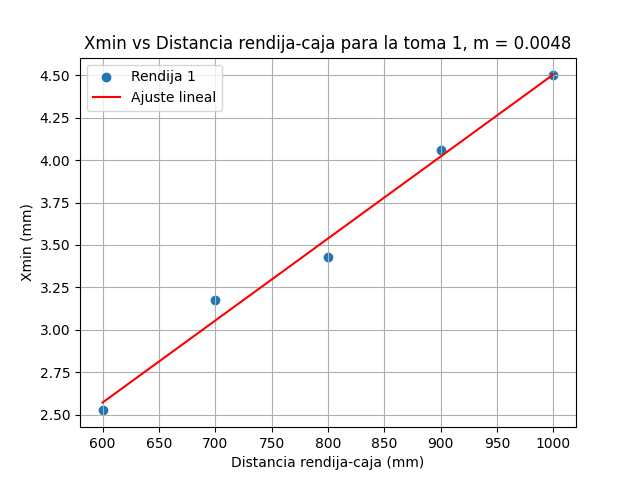
\includegraphics[width=0.4\textwidth]{fotos_practica/toma_1_rendija_simple.png}
    \caption{Gráfica de $X_{min}$ vs $D$ para la toma 1}
\end{figure}

\begin{figure}[H]
    \centering
    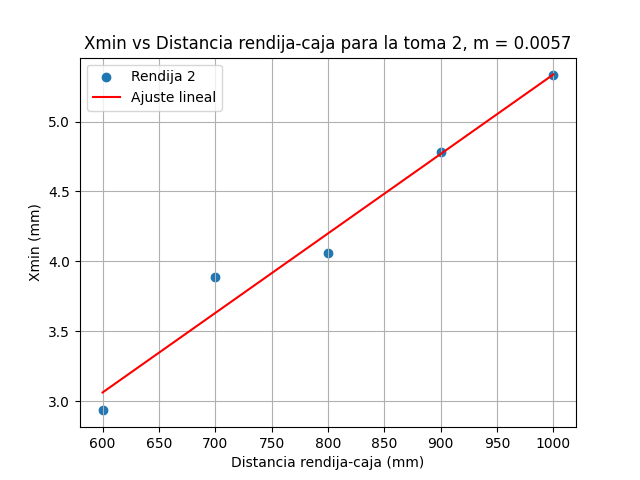
\includegraphics[width=0.4\textwidth]{fotos_practica/toma_2_rendija_simple.png}
    \caption{Gráfica de $X_{min}$ vs $D$ para la toma 2}
\end{figure}

\begin{figure}[H]
    \centering
    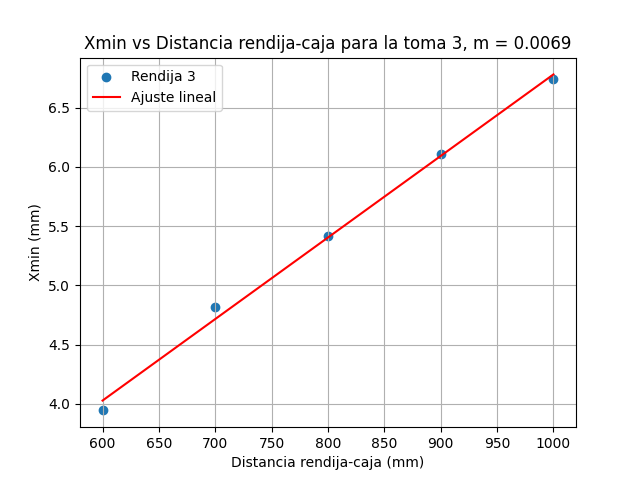
\includegraphics[width=0.4\textwidth]{fotos_practica/toma_3_rendija_simple.png}
    \caption{Gráfica de $X_{min}$ vs $D$ para la toma 3}
\end{figure}


\begin{figure}[H]
    \centering
    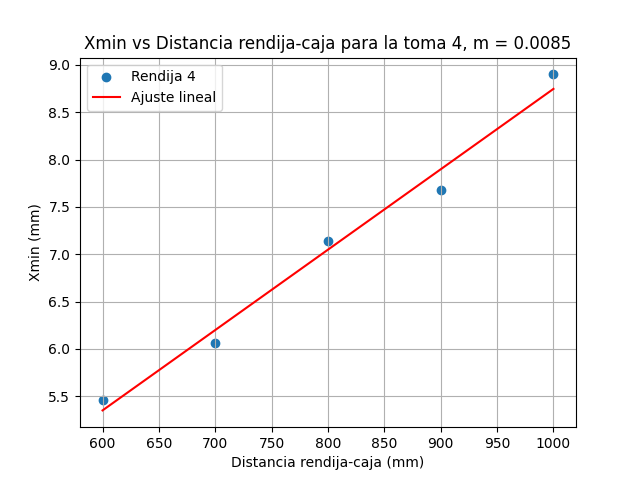
\includegraphics[width=0.4\textwidth]{fotos_practica/toma_4_rendija_simple.png}
    \caption{Gráfica de $X_{min}$ vs $D$ para la toma 4}
\end{figure}


\begin{figure}[H]
    \centering
    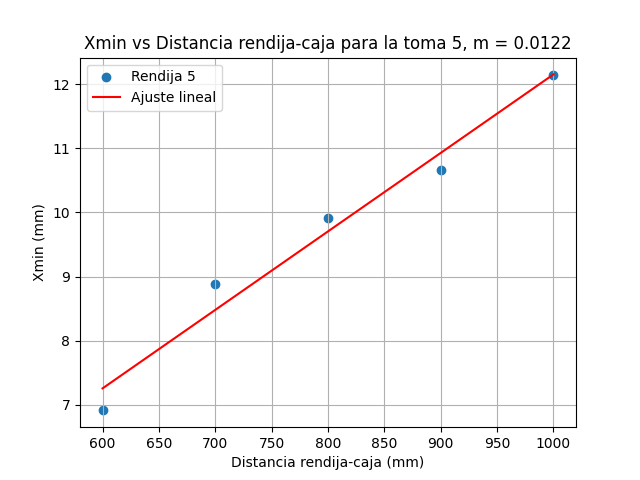
\includegraphics[width=0.4\textwidth]{fotos_practica/toma_5_rendija_simple.png}
    \caption{Gráfica de $X_{min}$ vs $D$ para la toma 5}
\end{figure}


\begin{figure}[H]
    \centering
    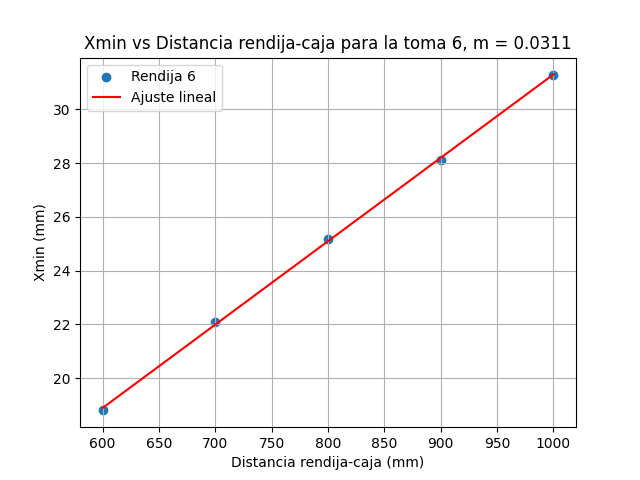
\includegraphics[width=0.4\textwidth]{fotos_practica/toma_6_rendija_simple.png}
    \caption{Gráfica de $X_{min}$ vs $D$ para la toma 6}
\end{figure}

\vspace{0.5cm}

Al hacer la media de los valores obtenidos para $m$, obtenemos que:
\begin{equation}
    \bar{m} = 0.012
\end{equation}

\vspace{0.5cm}


Y por tanto usando la relación $a = \frac{\lambda}{2 \bar{m}}$ obtenemos que la anchura de la rendija es de:
\begin{equation}
    a = 26.25 \, \mu\text{m}
\end{equation}

Podemos comparar este resultado obtenido con datos de las rendijas con rendijas similares en venta, en nuestro caso comparamos con la página \cite{ventus_rendijas} donde las rendijas tienen una anchura de 
$0.025 mm$, por tanto nuestro resultado se acerca mucho al real.
\subsection{Red de difracción}

En este caso se ha representado gráficamente la relación entre $X_{max}$ y $D$ para cada una de las 3 redes de difracción. Además, se ha realizado un ajuste lineal a cada una de las gráficas para obtener el valor de $p$ y así poder obtener el número de líneas por milímetro de cada red.
\begin{figure}[H]
    \centering
    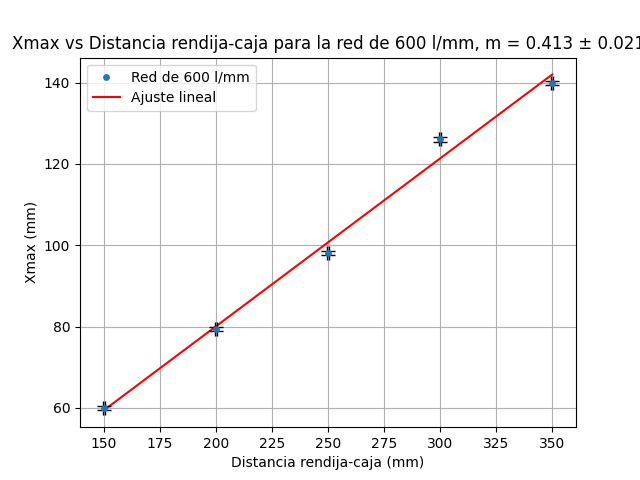
\includegraphics[width=0.4\textwidth]{fotos_practica/red_600.png}
    \caption{Gráfica de $X_{max}$ vs $D$ para la red de 600 líneas/mm}
\end{figure}

\begin{figure}[H]
    \centering
    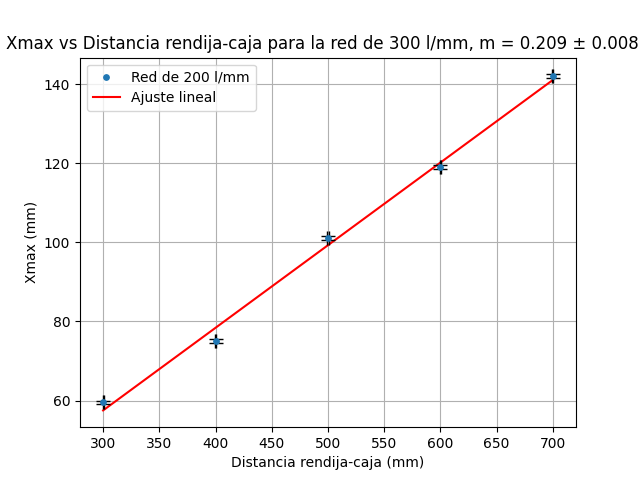
\includegraphics[width=0.4\textwidth]{fotos_practica/red_300.png}
    \caption{Gráfica de $X_{max}$ vs $D$ para la red de 300 líneas/mm}
\end{figure}

\begin{figure}[H]
    \centering
    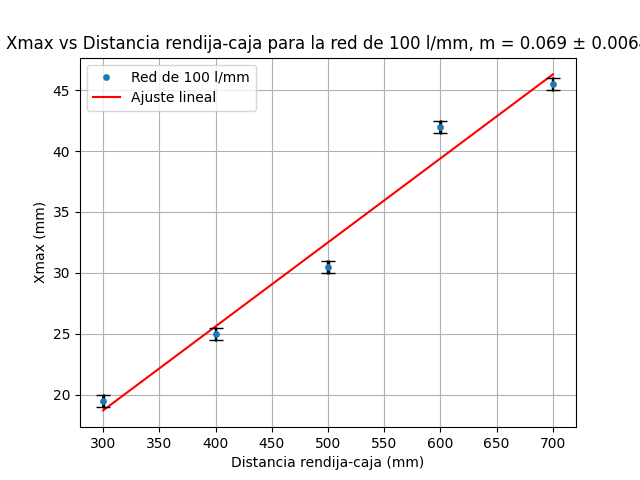
\includegraphics[width=0.4\textwidth]{fotos_practica/red_100.png}
    \caption{Gráfica de $X_{max}$ vs $D$ para la red de 100 líneas/mm}
\end{figure}

Con el análisis realizado, obtenemos que $p= \frac{m}{\lambda}$, con $\lambda = 650$ nm, primero antes de obtener los resultados debemos hacer el cálculo del error asociado:
\begin{equation}
    \Delta p = \left|\frac{\partial p}{\partial m}\right|\Delta m = \left|\frac{1}{\lambda}\right| \Delta m
\end{equation}
\begin{align}
    p_{600} = 635 \pm 32 \\
    p_{300} = 321 \pm 12 \\
    p_{100} = 106 \pm 9
\end{align}

Vemos pues que nuestros resultados, divergen ligeramente respecto al resultado teórico, pero al encontrarse en el mismo orden de magnitud, los errores pueden deberse a errores de 
calibración en la medida. 

\subsection{Espectroscopía de un gas}

Para este apartado utilizaremos el código programado para el apartado 6. Con ello, obtendremos las longitudes de onda representadas. Pasaremos en cada caso los datos a metros ya que es 
la unidad en la que esta basada el código. 

\begin{figure}[H]
    \centering
    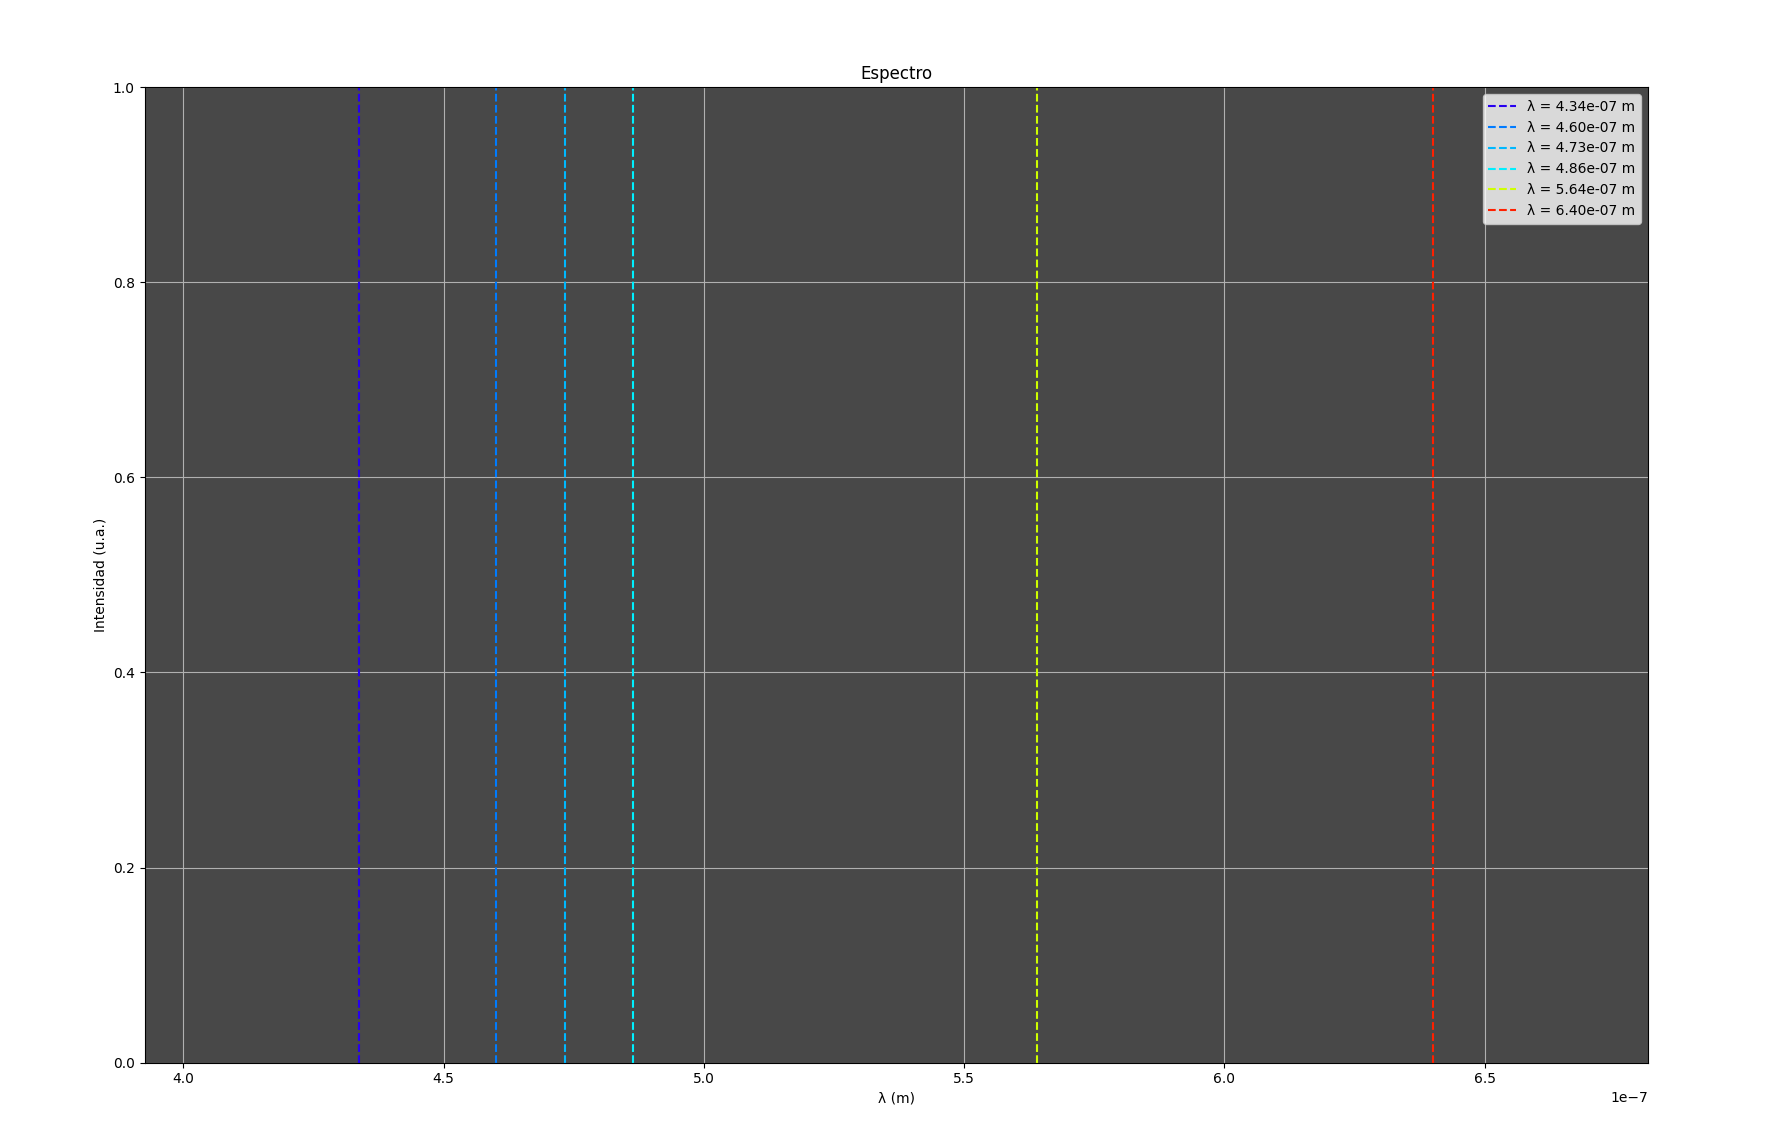
\includegraphics[width=0.4\textwidth]{fotos_practica/espectro600.png}
    \caption{Espectograma para los datos obtenidos para la red de 600 líneas/mm}
\end{figure}

\begin{figure}[H]
    \centering
    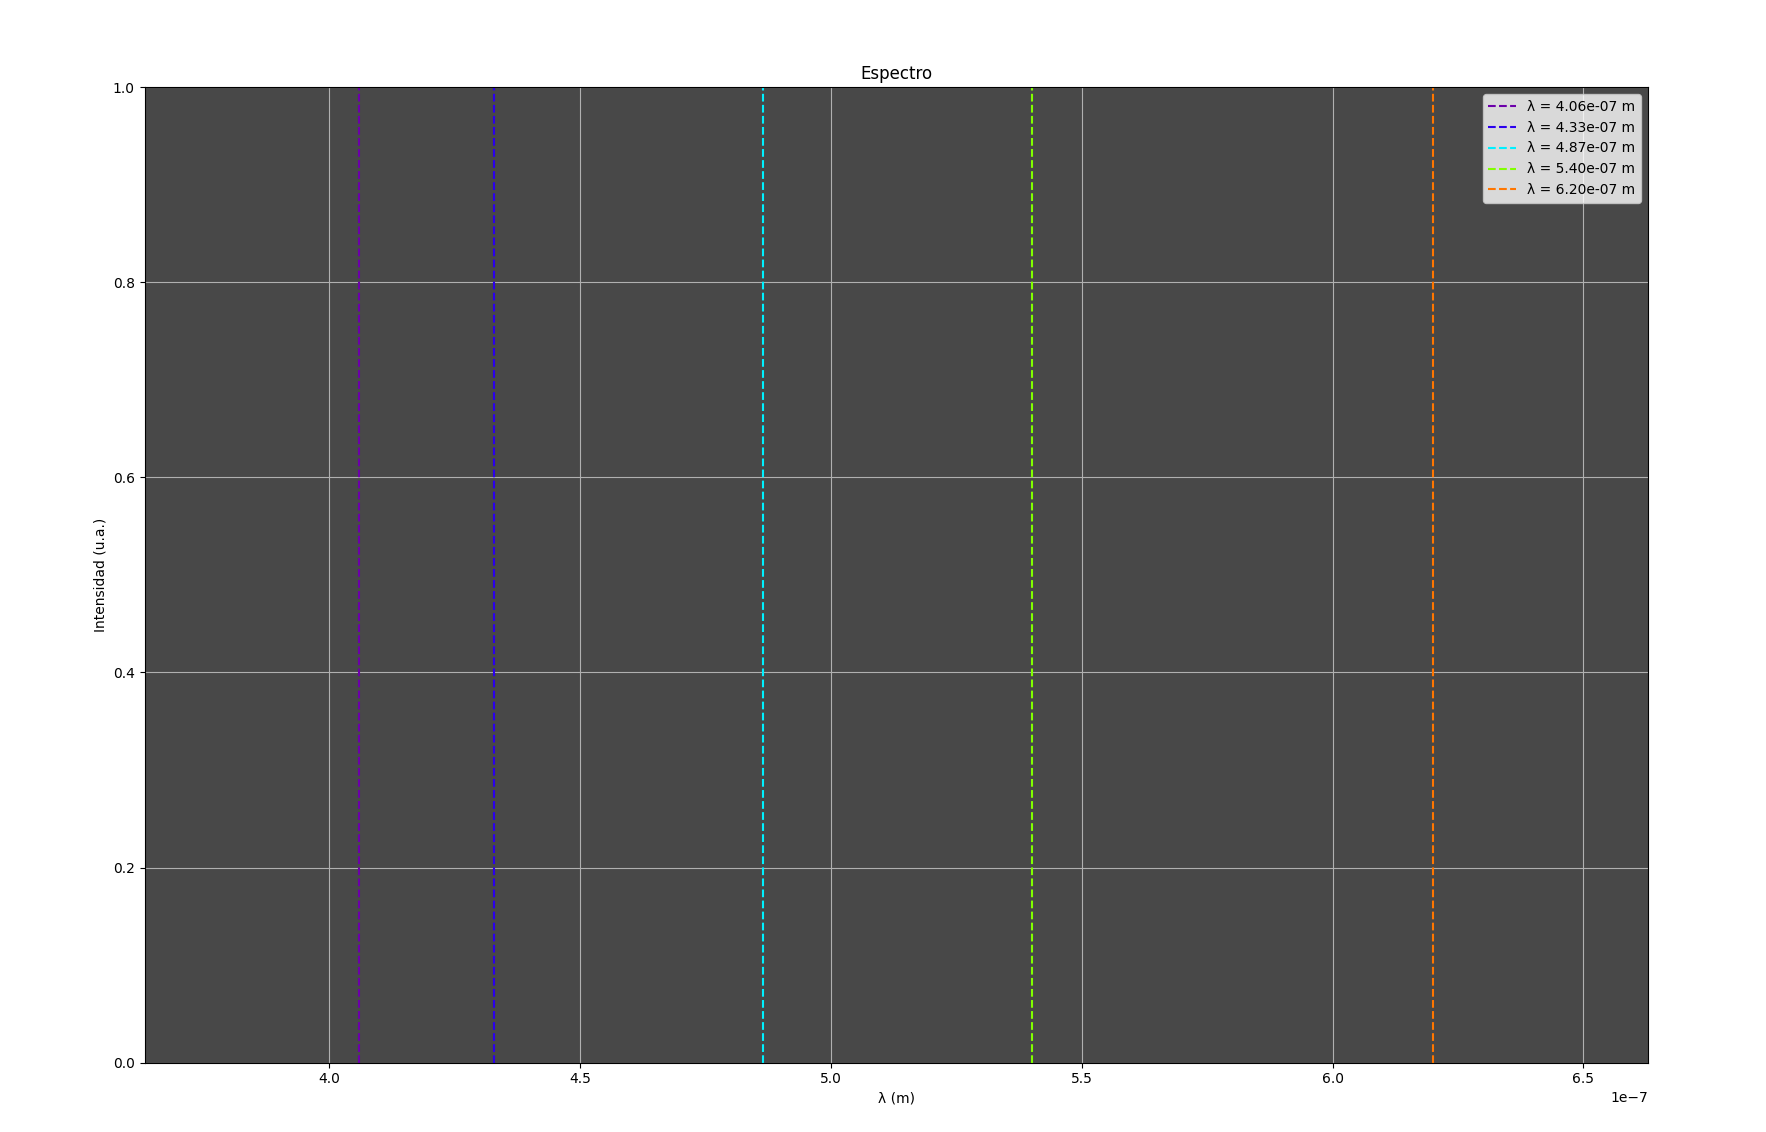
\includegraphics[width=0.4\textwidth]{fotos_practica/espectro_300.png}
    \caption{Espectograma para los datos obtenidos para la red de 300 líneas/mm}
\end{figure}

\begin{figure}
    \centering
    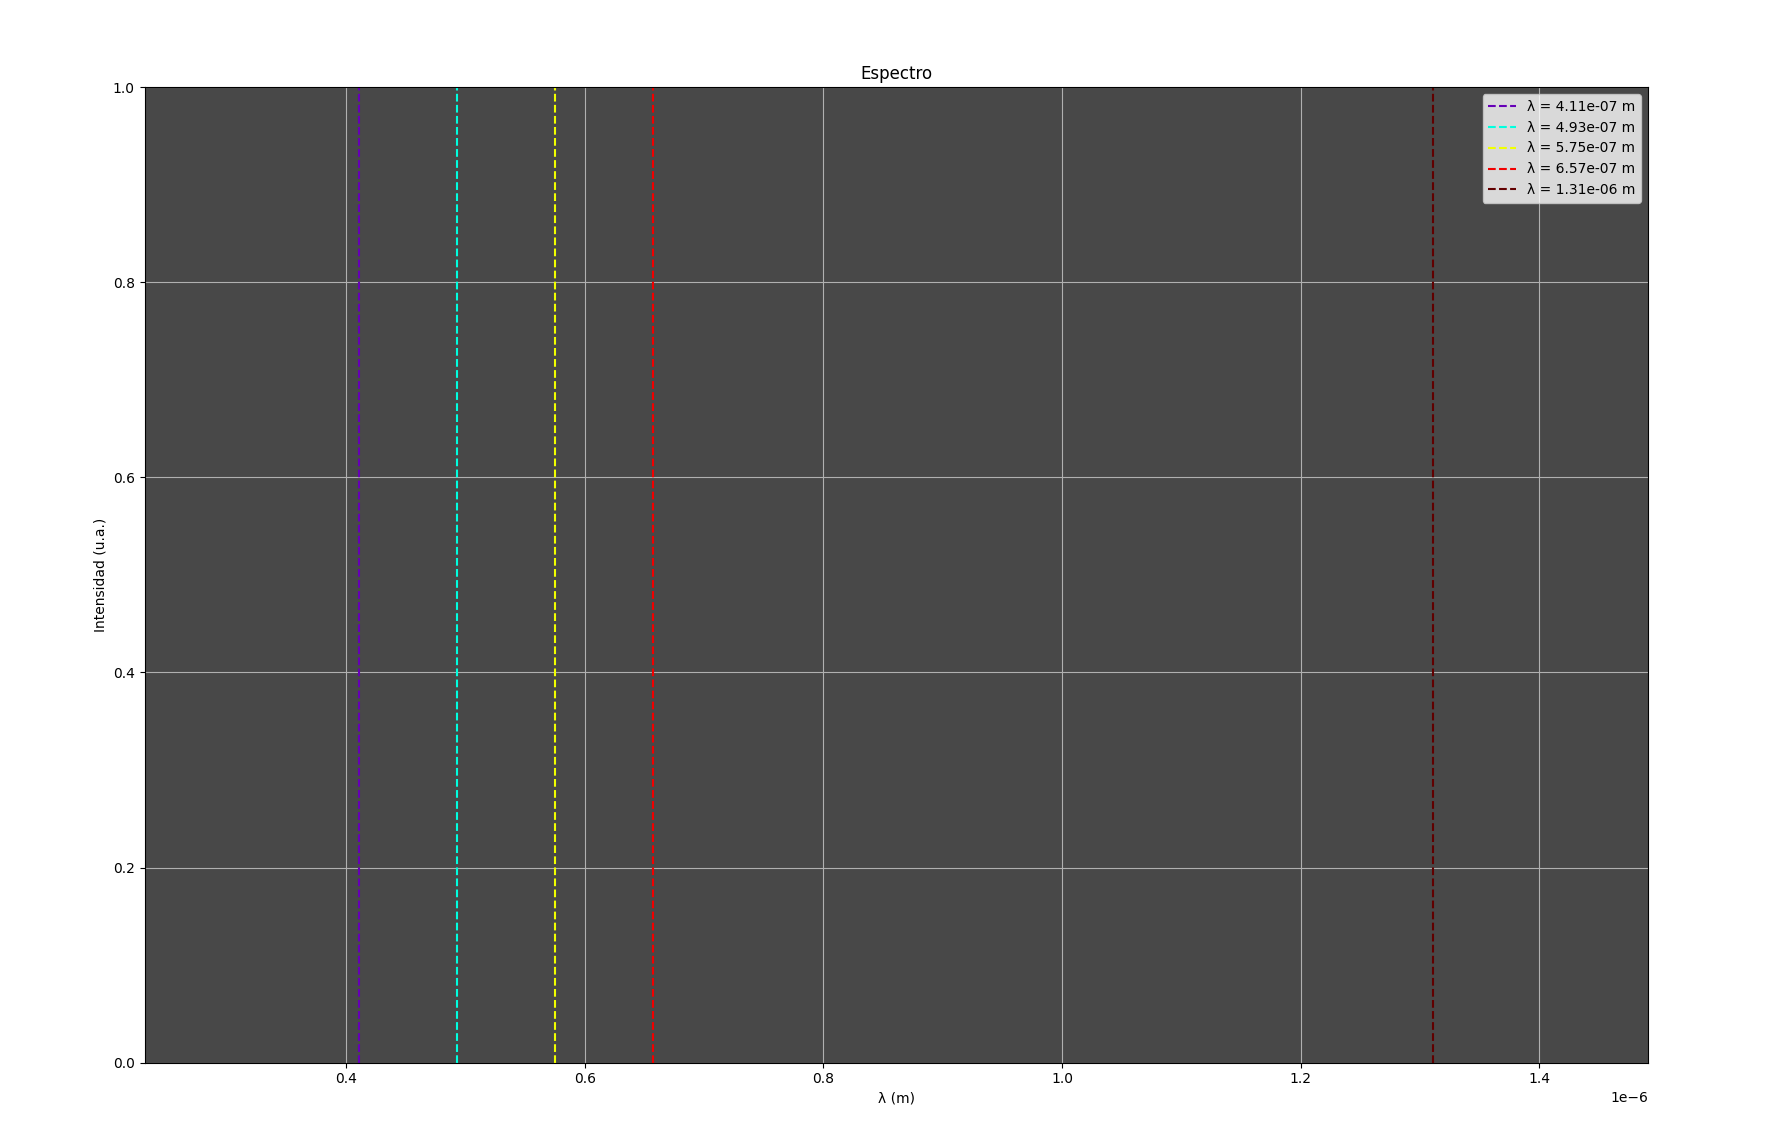
\includegraphics[width=0.4\textwidth]{fotos_practica/espectro_100.png}
    \caption{Espectograma para los datos obtenidos para la red de 100 líneas/mm}
\end{figure}
 
Para comparar con el Helio, utilizaremos la de 300 líneas/mm ya que es la que nos da mejores valores cercanos a los teóricos. Buscando encontramos el siguiente espectrograma, con los datos de $\lambda$
\cite{espectro_helio}:

\begin{table}[H]
    \centering
    \begin{tabular}{cccc}
        \hline
        $\lambda_{teo}$ & $\lambda_{exp}$  & $\lambda_{tablas}$ & $\Delta \lambda_{tablas}$ \\
        \hline

        438             &    434           & 422.319            & $\pm 3e-05$ \\
        443             &    460           & 450.296            & $\pm 3e-05$ \\
        471             &    473           & 456                & $\pm 3e-05$ \\
        492             &    486           & 506.146            & $\pm 3e-05$\\
        587             &    563           & 561.841            & $\pm 3e-05$\\
        667             &    640           & 645.058            & $\pm 3e-05$\\
        \hline          
    \end{tabular}
    
\end{table}

En esta tabla podemos ver que nuestros resultados a través del código y el cálculo de tablas se acercan bastante al resultado deseado. Si bien, faltan 2 espectros
si mencionados en la página citada.


Por último incluimos en un apéndice el código pedido en la parte computacional, aunque también será aportado el archivo .py junto al informe.

\section{Conclusiones}
En primer lugar, la determinación de la anchura de la rendija simple arrojó un valor de $26.25\,\mu\text{m}$, lo cual muestra una excelente 
concordancia con los valores comerciales que fueron encontrados en la página citada \cite{ventus_rendijas}, ($0.025\,\text{mm}$), validando la precisión del modelo de Fraunhofer y 
del método de ajuste lineal usado para la rendija simple en este caso.

En cuanto a las redes de difracción, los parámetros de red obtenidos ($p$) se mantuvieron en el orden de magnitud esperado. 
Aunque se observaron ligeras desviaciones respecto a los valores nominales (especialmente en la red de 600 líneas/mm), estas son atribuibles a incertidumbres sistemáticas en 
la medición de distancias y posibles errores de paralaje en la toma de datos.

Finalmente, el estudio espectroscópico del helio permitió identificar sus líneas de emisión características. La red de 300 líneas/mm resultó ser la más eficaz para este propósito, ofreciendo longitudes de onda muy cercanas a las tabuladas
en la página \cite{espectro_helio}. Esto confirma la potencia de la difracción como herramienta analítica en la identificación de elementos químicos. 


\vspace{0.5cm}
Para ver todo el análisis de datos realizado por los alumnos, se habilita este enlace al repositorio de github donde están todos los archivos de práctias: 
\cite{2026experimental}

\section{Referencias}

\printbibliography

\end{document}